\chapter{User Interface Design} \label{chap4}
Here are presented some mockups that represent an idea of the structure of the application pages.

\section{Splash Screen and Registration \& Login Pages}
These mockups show an idea of the \textit{Splash Screen} and \textit{Registration \& Login} pages of the application. The \textit{Registration \& Login Page} allow the user of the application to register as a user of the service and this can be performed via the custom application functionality or via external providers.\\

\begin{figure}[!htbp]
  \centering
  \begin{minipage}[b]{0.45\textwidth}
    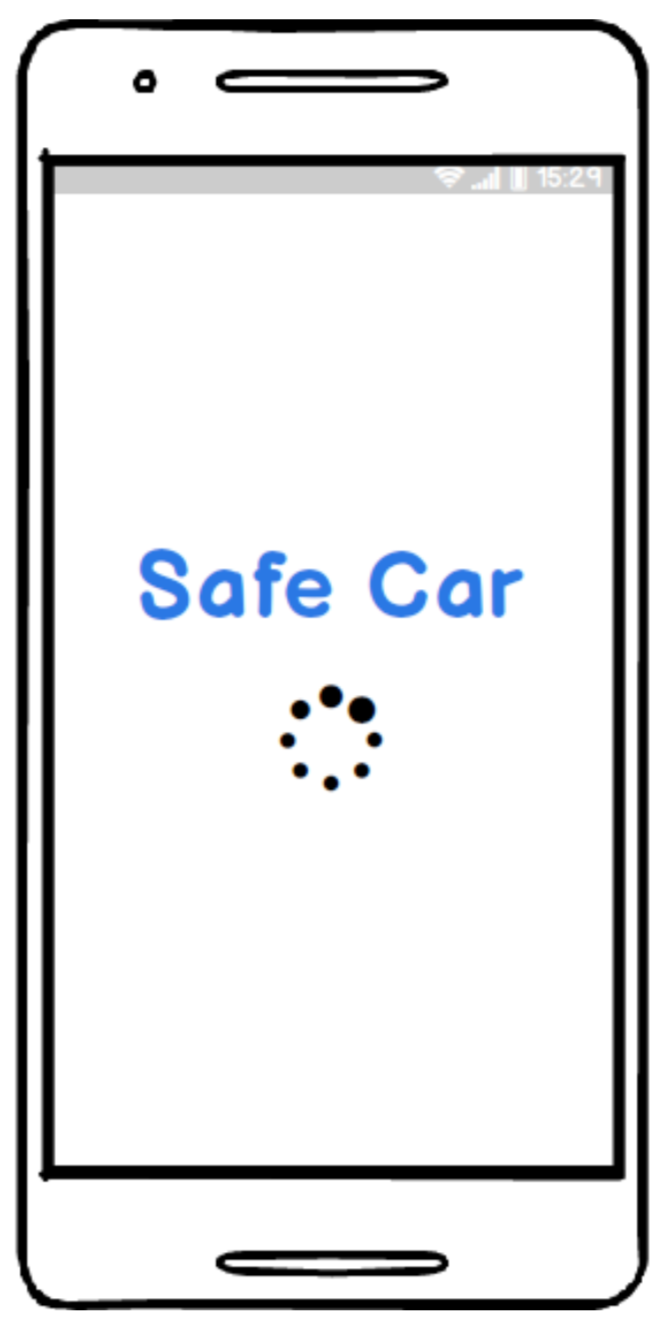
\includegraphics[width=\textwidth]{cpt/img/SplashScreen.png}
    \caption{Splash Screen}
  \end{minipage}
  \hfill
  \begin{minipage}[b]{0.45\textwidth}
    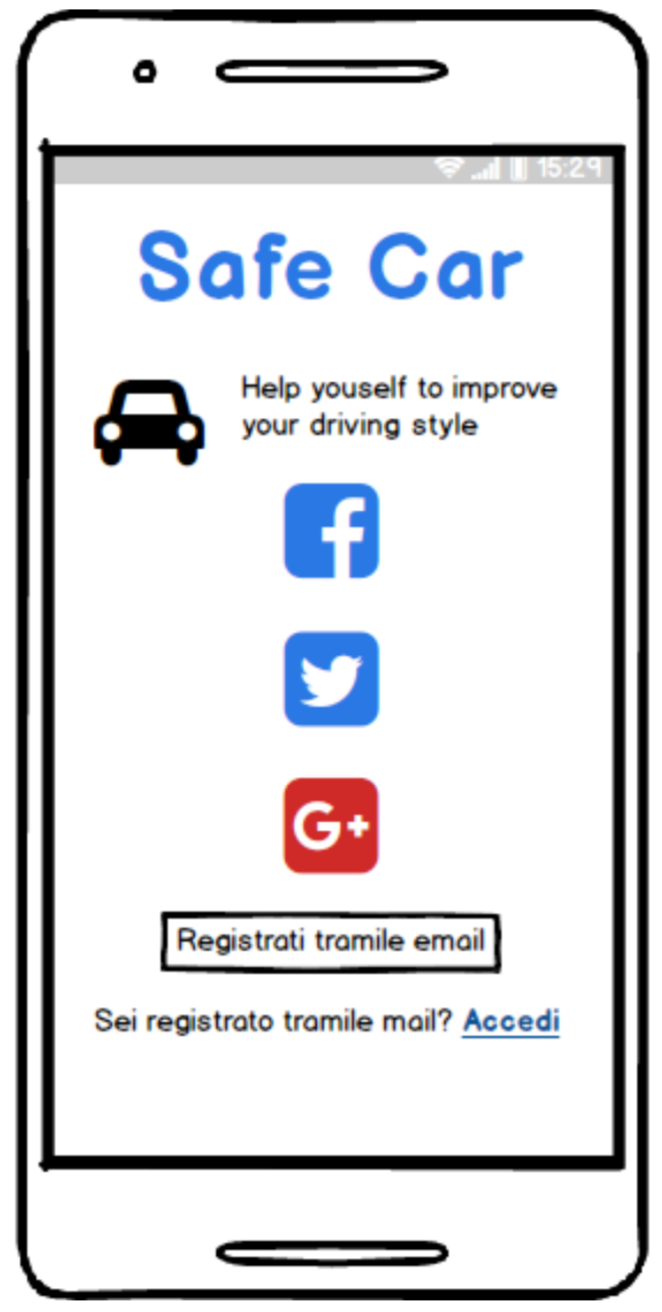
\includegraphics[width=\textwidth]{cpt/img/Login.png}
    \caption{Registration \& Login}
  \end{minipage}
\end{figure}

\clearpage
\section{Home Page}
These mockups show an idea of the \textit{Home Page} of the application. The \textit{Home Page} presents a \textit{TabView} through which the user can navigate in order to inspect his history trips and a \textit{Navigation Drawer Menu} through which the user can reach other pages of the application.\\

\begin{figure}[htbp]
\centering
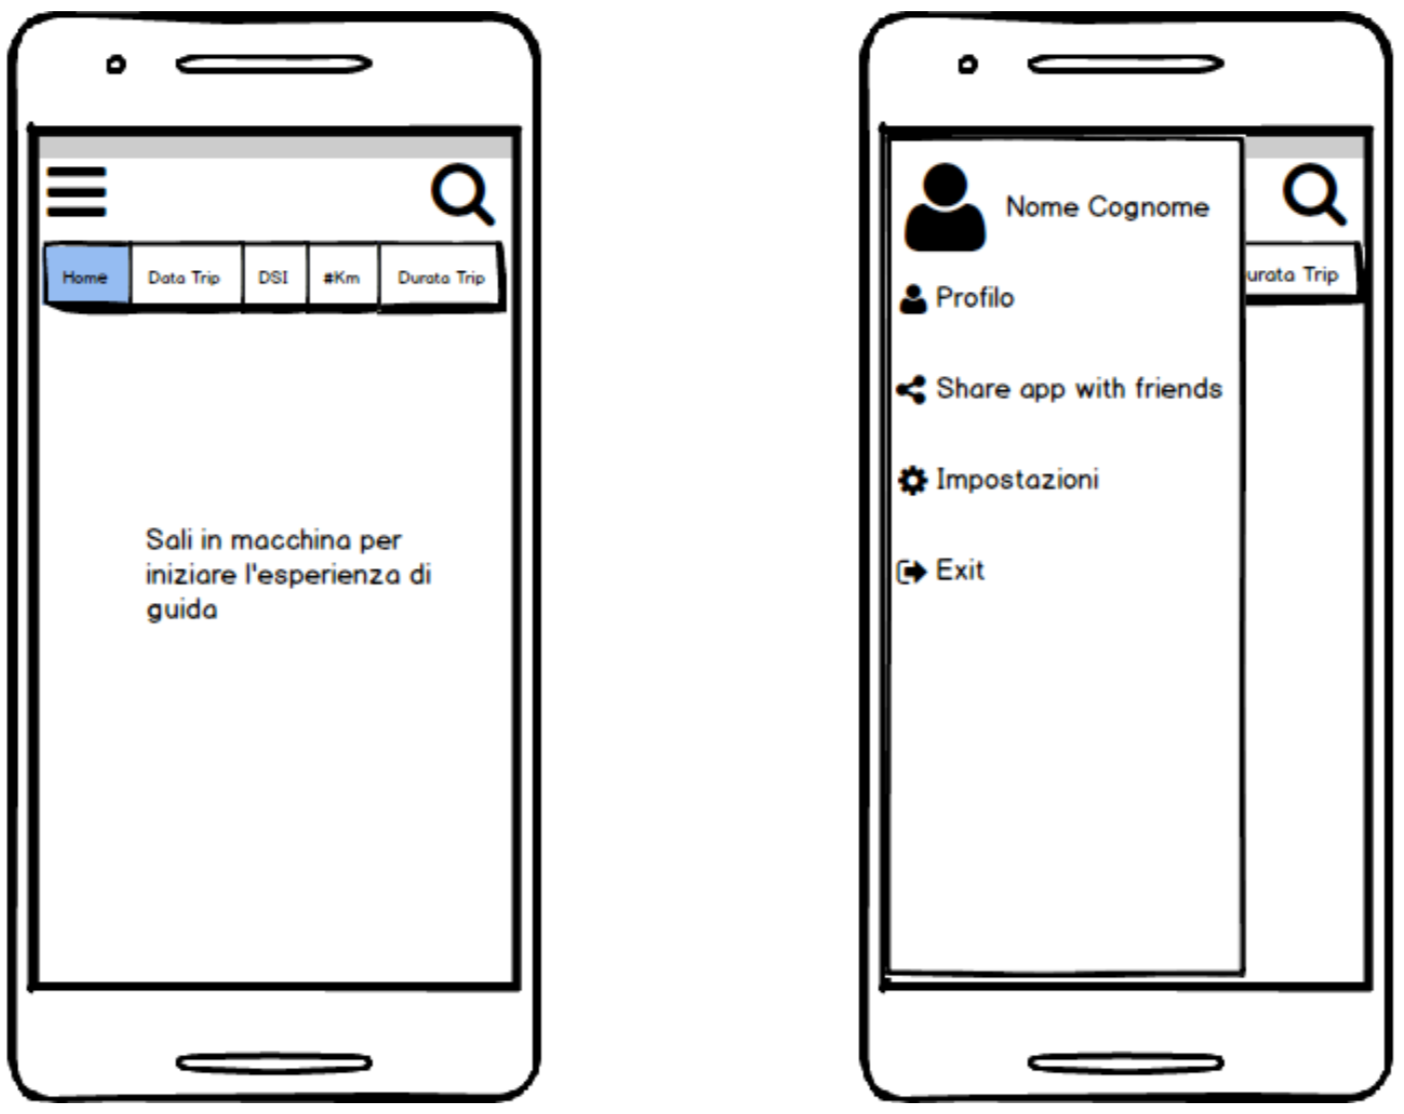
\includegraphics[width=\textwidth]{cpt/img/HomePage.png}
\caption{Home Page}
\end{figure}

\clearpage
\section{During Trip Page}
These mockups show an idea of the \textit{During Trip Page} of the application. The \textit{During Trip Page} presents a \textit{View} where \textit{Hints} produced by the application are loaded and viewable by the user. The user can interact with the application using two buttons: the first one is a \textit{Pause/Resume} button which allow the user to pause the trip, without stopping it, if he wants to take a break from the driving session and, then, resume it; the second one, instead, is a \textit{Stop} button which allow the user to end the driving experience.\\

\begin{figure}[htbp]
\centering
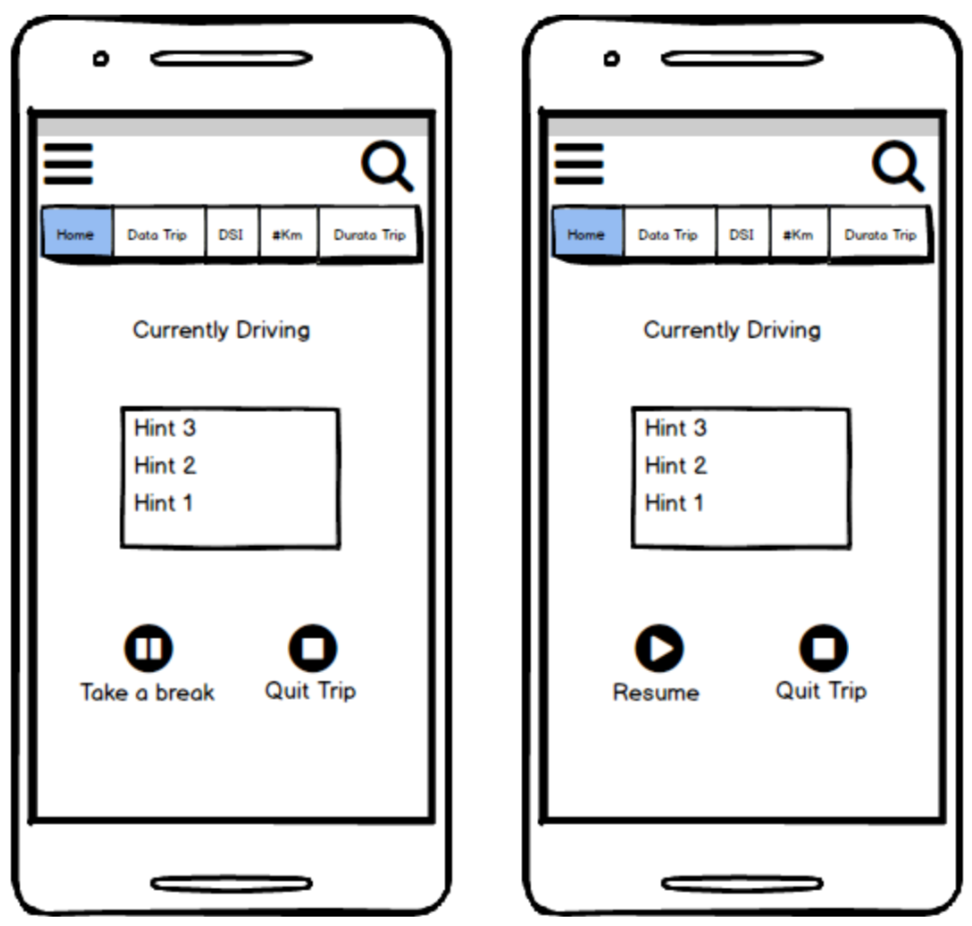
\includegraphics[width=\textwidth]{cpt/img/DuringTrip.png}
\caption{During Trip}
\end{figure}

\clearpage
\section{Report Page}
This mockup show an idea of the \textit{Report Page} of the application. The \textit{Report Page} is showed when the user inspect one of his history trips or when he complete a driving session pushing the \textit{Stop} button. This page allow the user to see all the details about his trip including data like: the trip's date, duration and length, the DSI score and the path he made.\\

\begin{figure}[htbp]
\centering
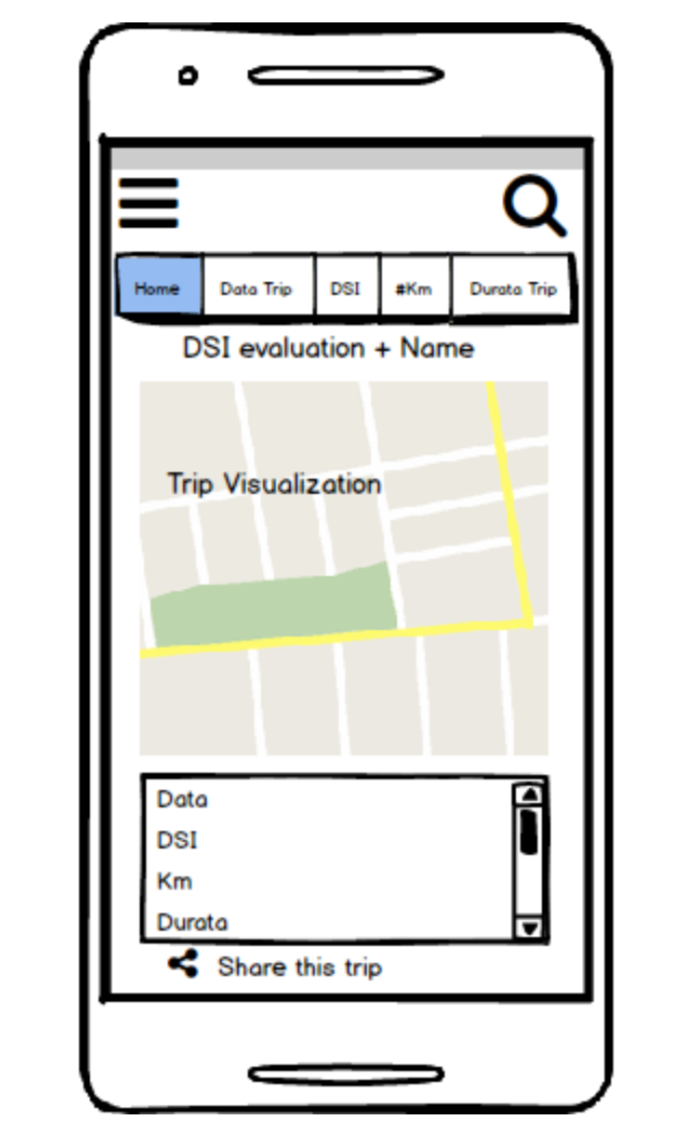
\includegraphics[width=0.7\textwidth]{cpt/img/ReportPage.png}
\caption{Report Page}
\end{figure}

\clearpage
\section{Profile Page}
These mockups show an idea of the \textit{Profile Page} of the application. The \textit{Profile Page} shows information about the user like his name, surname, email address, driver level and also some badges that he can unlock meeting specific conditions. Each badge is clickable and let the user know about its locked/unlocked status.\\

\begin{figure}[htbp]
\centering
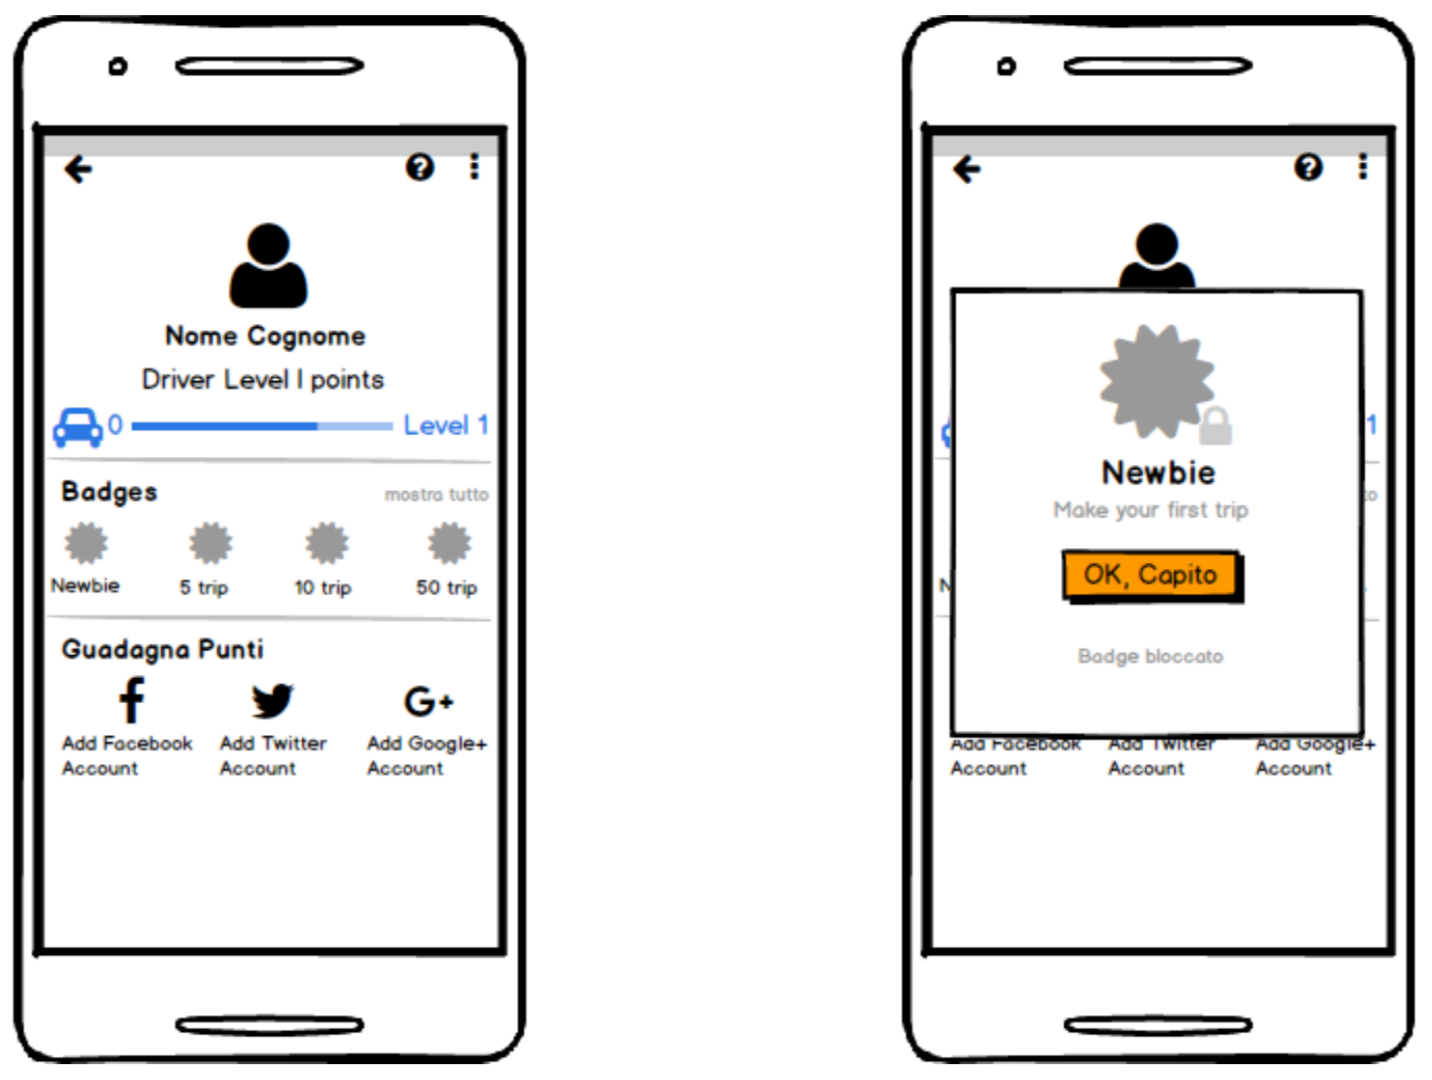
\includegraphics[width=\textwidth]{cpt/img/ProfilePage.png}
\caption{Profile Page}
\end{figure}

\clearpage
\section{Settings Page}
This mockup show an idea of the \textit{Settings Page} of the application. The \textit{Settings Page} allow the user to manage some settings of the application like push notifications and smart objects. This page also allow the user to see some info about the application and send feedback in order to improve it.\\

\begin{figure}[htbp]
\centering
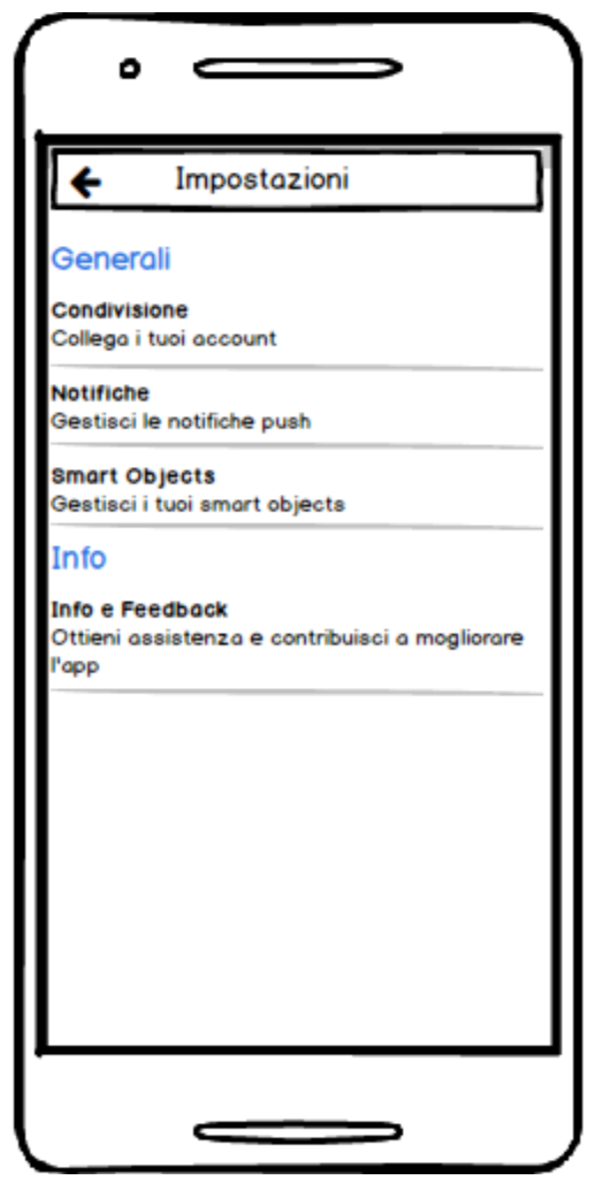
\includegraphics[width=0.55\textwidth]{cpt/img/SettingsPage.png}
\caption{Settings Page}
\end{figure}

\clearpage
\section{Smart Objects Page}
These mockups show an idea of the \textit{Smart Objects Pages} of the application. The \textit{Smart Objects Pages} allow the user to manage smart objects which are necessary for the application. Using a bluetooth scanner the user can pair his device with a plug used to retrieve relevant information about the current driving session and he can also manage all the paired plugs, inspecting or deleting them.\\

\begin{figure}[htbp]
\centering
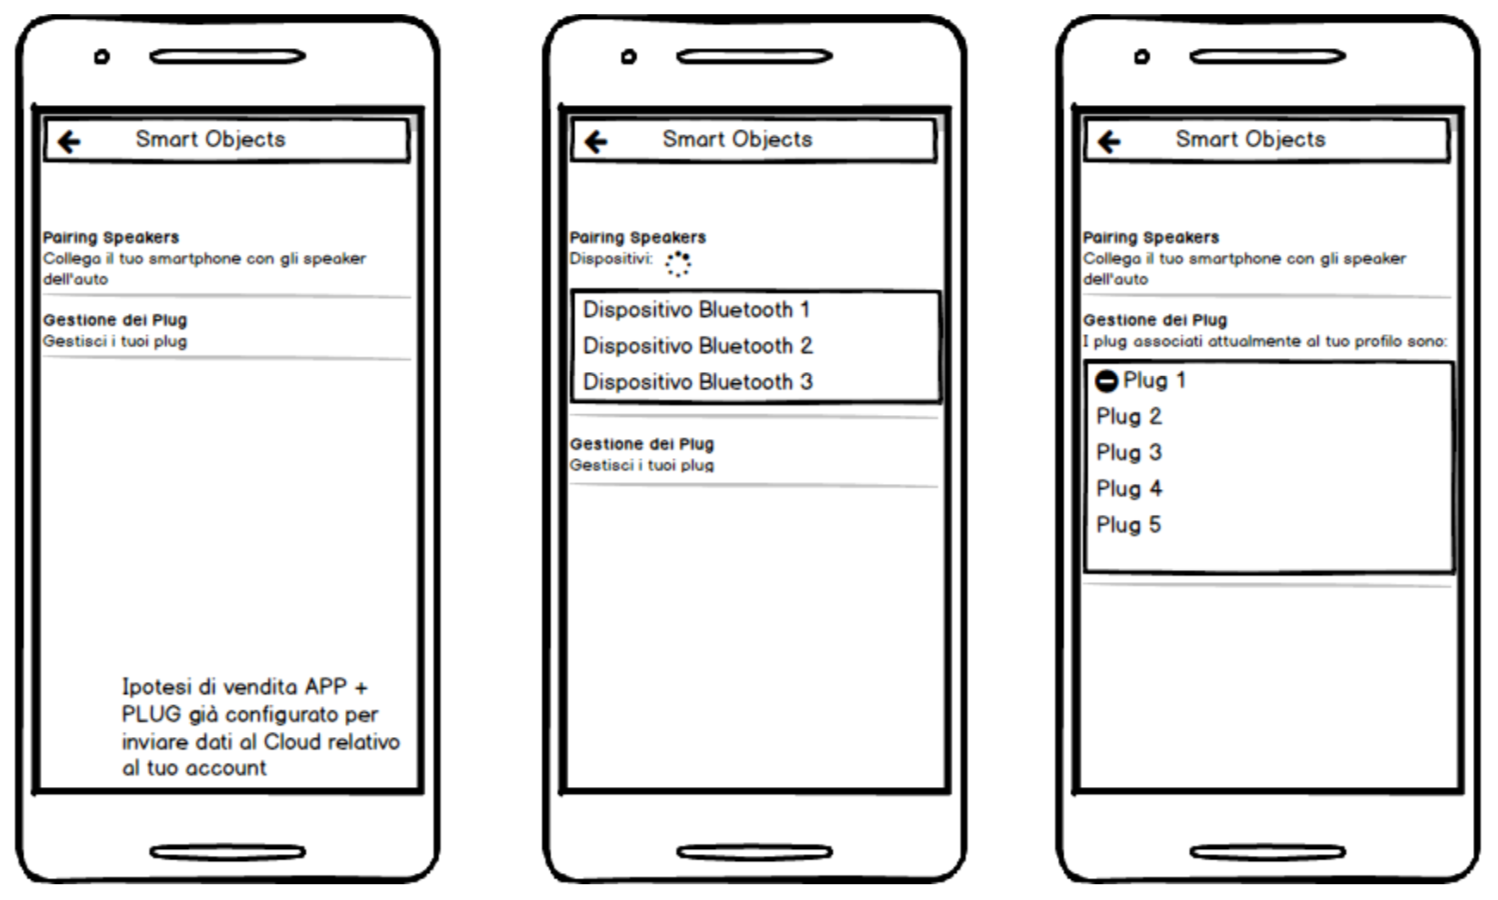
\includegraphics[width=\textwidth]{cpt/img/SmartObjectsPage.png}
\caption{Smart Objects Pages}
\end{figure}